\documentclass[12pt, letterpaper]{article}
\usepackage{fancyhdr}
\usepackage{glossaries}
\usepackage{graphicx}
\usepackage[hidelinks]{hyperref}
\usepackage[utf8]{inputenc}
\usepackage{makecell}

\pagestyle{fancy}
\fancyhf{}
\lhead{DICOM Conformance Statement}
\rhead{Slim v0.11.2}
\lfoot{MGH Pathology}
\rfoot{Page \thepage}
\renewcommand{\headrulewidth}{0.5pt}
\renewcommand{\footrulewidth}{0.5pt}

\title{Slim v0.11.2}
\author{MGH Pathology}
\date{October 6, 2022}

\hyphenation{DICOM}

\def\UrlBreaks{\do\/\do-}

\setlength{\parindent}{0em}
\setlength{\parskip}{0.5em}

\newglossaryentry{AE}{
    name=AE,
    description=Application Entity
}
\newglossaryentry{AET}{
    name=AET,
    description=Application Entity Title
}
\newglossaryentry{API}{
    name=API,
    description=Application Programming Interface
}
\newglossaryentry{CAD}{
    name=CAD,
    description=Computer Aided Detection
}
\newglossaryentry{DICOM}{
    name=DICOM,
    description=Digital Imaging and Communications in Medicine
}
\newglossaryentry{DNS}{
    name=DNS,
    description=Domain Name System
}
\newglossaryentry{HIS}{
    name=HIS,
    description=Hospital Information System
}
\newglossaryentry{HL7}{
    name=HL7,
    description=Health Level 7 Standard
}
\newglossaryentry{HTTP}{
    name=HTTP,
    description=Hyptertext Transfer Protocol
}
\newglossaryentry{ICC}{
    name=ICC,
    description=International Color Consortium
}
\newglossaryentry{IOD}{
    name=IOD,
    description=Information Object Definition
}
\newglossaryentry{IPv4}{
    name=IPv4,
    description=Internet Protocol version 4
}
\newglossaryentry{IPv6}{
    name=IPv6,
    description=Internet Protocol version 6
}
\newglossaryentry{ISO}{
    name=ISO,
    description=International Organization for Standards
}
\newglossaryentry{JPEG}{
    name=JPEG,
    description=Joint Photographic Experts Group
}
\newglossaryentry{LDAP}{
    name=LDAP,
    description=Lightweight Directory Access Protocol
}
\newglossaryentry{LIS}{
    name=LIS,
    description=Laboratory Information System
}
\newglossaryentry{NPM}{
    name=NPM,
    description=Node Package Manager
}
\newglossaryentry{O}{
    name=O,
    description=Optional (Key Attribute)
}
\newglossaryentry{OSI}{
    name=OSI,
    description=Open Systems Interconnection
}
\newglossaryentry{PACS}{
    name=PACS,
    description=Picture Archiving and Communication System
}
\newglossaryentry{PNG}{
    name=PNG,
    description=Portable Network Graphics
}
\newglossaryentry{QIDO-RS}{
    name=QIDO-RS,
    description=Search transaction of the DICOM Web Studies Service
}
\newglossaryentry{R}{
    name=R,
    description=Required (Key Attribute)
}
\newglossaryentry{REST}{
    name=REST,
    description=Representational State Transfer
}
\newglossaryentry{SCP}{
    name=SCP,
    description=Service Class Provider
}
\newglossaryentry{SCU}{
    name=SCU,
    description=Service Class User
}
\newglossaryentry{SM}{
    name=SM,
    description=Slide Microscopy
}
\newglossaryentry{SOP}{
    name=SOP,
    description=Service-Object Pair
}
\newglossaryentry{SR}{
    name=SR,
    description=Structured Reporting
}
\newglossaryentry{TCPIP}{
    name=TCP/IP,
    description=Transmission Control Protocol/Internet Protocol
}
\newglossaryentry{U}{
    name=U,
    description=Unique (Key Attribute)
}
\newglossaryentry{UML}{
    name=UML,
    description=Unified Modeling Language
}
\newglossaryentry{VL}{
    name=VL,
    description=Visible Light
}
\newglossaryentry{VR}{
    name=VR,
    description=Value Representation
}
\newglossaryentry{WADO-RS}{
    name=WADO-RS,
    description=Retrieve transaction of the DICOM Web Studies Service
}

\renewcommand{\glossarysection}[2][]{}

\makeglossary%


\begin{document}

\begin{titlepage}
    \maketitle
\end{titlepage}


\section*{Conformance Statement Overview}

\emph{Slim} is a dynamic single-page application that allows users to interactively display \gls{DICOM} \gls{VL} Whole Slide Microscopy Image instances in a web browser.

\emph{Slim} relies on the JavaScript \emph{dicom-microscopy-viewer} library to display digitial images and related information to the user.
\emph{Slim} as well as the \emph{dicom-microscopy-viewer} internally use the JavaScript \emph{dicomweb-client} library to programmatically search for and retrieve data from a \gls{PACS} using the Search and Retrieve transactions of the \gls{DICOM} Web Studies Service, respectively.

\begin{table}[h!]
    \center
    \begin{tabular}{ |l|c|c| }
        \hline
        Service & \thead{User of Service \\ (User Agent)} & \thead{Provider of Service \\ (Origin Server)} \\
        \hline\hline
        \multicolumn{3}{|l|}{Studies Service} \\
        \hline
        Retrieve transaction (WADO-RS) & Yes & No \\
        \hline
        Search transaction (QIDO-RS) & Yes & No \\
        \hline
    \end{tabular}
    \caption{DICOM Web Services}
    \label{table:1}
\end{table}

\tableofcontents

\section{Introduction}

\subsection{Revision History}

\begin{table}
    \begin{tabular}{ |c|c|c|c| }
        \hline
        Document Version & Revision Date & Revision Author\\
        \hline
        v0.11.2 & October, 2022 & Markus D. Herrmann \\
        \hline
    \end{tabular}
\end{table}

\subsection{Audience}

This document is written for the people that need to understand how \emph{Slim} will integrate into their healthcare facility.
This includes both those responsible for overall imaging network policy and architecture, as well as integrators who need to have a detailed understanding of the \gls{DICOM} features of the product.
This document contains some basic \gls{DICOM} definitions so that any reader may understand how this product implements \gls{DICOM} features.
However, integrators are expected to fully understand all the \gls{DICOM} terminology, how the tables in this document relate to the product's functionality, and how that functionality integrates with other devices that support compatible \gls{DICOM} features.

\subsection{Remarks}

The scope of this \gls{DICOM} Conformance Statement is to facilitate integration between \emph{Slim} and other \gls{DICOM} products.
The Conformance Statement should be read and understood in conjunction with the \gls{DICOM} Standard.
\gls{DICOM} by itself does not guarantee interoperability.
The Conformance Statement does, however, facilitate a first-level comparison for interoperability between different applications supporting compatible \gls{DICOM} functionality.

This Conformance Statement is not supposed to replace validation with other \gls{DICOM} equipment to ensure proper exchange of intended information.
In fact, the user should be aware of the following important issues:

\begin{itemize}
    \item The comparison of different Conformance Statements is just the first step towards assessing interconnectivity and interoperability between the product and other \gls{DICOM} conformant equipment.

    \item Test procedures should be defined and executed to validate the required level of interoperability with specific compatible \gls{DICOM} equipment, as established by the healthcare facility.
\end{itemize}

\subsection{Terms and Definitions}

Informal definitions are provided for the following terms used in this Conformance Statement.
The \gls{DICOM} Standard is the authoritative source for formal definitions of these terms.

\begin{description}

    \item [Abstract Syntax] The information agreed to be exchanged between applications, generally equivalent to a Service/Object Pair (\gls{SOP}) Class.
        Examples: Verification \gls{SOP} Class, Modality Worklist Information Model Find \gls{SOP} Class, Computed Radiography Image Storage \gls{SOP} Class.

    \item [Application Entity (AE)] An end point of a \gls{DICOM} information exchange, including the \gls{DICOM} network or media interface software; i.e., the software that sends or receives \gls{DICOM} information objects or messages.
        A single device may have multiple Application Entities.

    \item [Application Entity Title (AET)] The externally known name of an Application Entity, used to identify a \gls{DICOM} application to other \gls{DICOM} applications on the network. 

    \item [Application Context] The specification of the type of communication used between Application Entities.
        Example: \gls{DICOM} network protocol.

    \item [Association] A network communication channel set up between Application Entities.

    \item [Attribute] A unit of information in an object definition; a data element identified by a tag.
        The information may be a complex data structure (Sequence), itself composed of lower level data elements.
        Examples: Patient ID (0010,0020), Accession Number (0008,0050), Photometric Interpretation (0028,0004), Procedure Code Sequence (0008,1032).

    \item [Information Object Definition (IOD)] The specified set of Attributes that comprise a type of data object; does not represent a specific instance of the data object, but rather a class of similar data objects that have the same properties.
        The Attributes may be specified as Mandatory (Type 1), Required but possibly unknown (Type 2), or Optional (Type 3), and there may be conditions associated with the use of an Attribute (Types 1C and 2C).
        Examples: MR Image \gls{IOD}, CT Image \gls{IOD}, Print Job \gls{IOD}.\@

    \item [Joint Photographic Experts Group (JPEG)] A set of standardized image compression techniques, available for use by \gls{DICOM} applications.

    \item [Media Application Profile] The specification of \gls{DICOM} information objects and encoding exchanged on removable media (e.g., CDs).

    \item [Module] A set of Attributes within an Information Object Definition that are logically related to each other.
        Example: Patient Module includes Patient Name, Patient ID, Patient Birth Date, and Patient Sex.

    \item [Negotiation] First phase of Association establishment that allows Application Entities to agree on the types of data to be exchanged and how that data will be encoded. 

    \item [Presentation Context] The set of \gls{DICOM} network services used over an Association, as negotiated between Application Entities; includes Abstract Syntaxes and Transfer Syntaxes.

    \item [Protocol Data Unit (PDU)] A packet (piece) of a \gls{DICOM} message sent across the network. Devices must specify the maximum size packet they can receive for \gls{DICOM} messages.

    \item [Security Profile] A set of mechanisms, such as encryption, user authentication, or digital signatures, used by an Application Entity to ensure confidentiality, integrity, and/or availability of exchanged \gls{DICOM} data.

    \item [Service Class Provider (SCP)] Role of an Application Entity that provides a \gls{DICOM} network service; typically, a server that performs operations requested by another Application Entity (Service Class User).
        Examples: Picture Archiving and Communication System (image storage \gls{SCP}, and image query/retrieve \gls{SCP}), Radiology Information System (modality worklist \gls{SCP}).

    \item [Service Class User (SCU)] Role of an Application Entity that uses a \gls{DICOM} network service; typically, a client. 
        Examples: imaging modality (image storage \gls{SCU}, and modality worklist \gls{SCU}), imaging workstation (image query/retrieve \gls{SCU}).

    \item [Service/Object Pair Class (SOP Class)] The specification of the network or media transfer (service) of a particular type of data (object); the fundamental unit of \gls{DICOM} interoperability specification.
        Examples: Ultrasound Image Storage Service, Basic Grayscale Print Management.

    \item [Service/Object Pair Instance (SOP Instance)] An information object; a specific occurrence of information exchanged in a \gls{SOP} Class.
        Examples: a specific x-ray image.

    \item [Tag] A 32-bit identifier for a data element, represented as a pair of four digit hexadecimal numbers, the ``group'' and the ``element''. If the ``group'' number is odd, the tag is for a private (manufacturer-specific) data element.
        Examples: (0010,0020) [Patient ID], (07FE,0010) [Pixel Data], (0019,0210) [private data element].

    \item [Transfer Syntax] The encoding used for exchange of \gls{DICOM} information objects and messages.
        Examples: JPEG compressed (images), little endian explicit value representation.

    \item [Unique Identifier (UID)] A globally unique ``dotted decimal'' string that identifies a specific object or a class of objects; an ISO-8824 Object Identifier.
        Examples: Study Instance UID, SOP Class UID, SOP Instance UID.\@

    \item [Value Representation (VR)] The format type of an individual \gls{DICOM} data element, such as text, an integer, a person's name, or a code.
        \gls{DICOM} information objects can be transmitted with either explicit identification of the type of each data element (Explicit \gls{VR}), or without explicit identification (Implicit \gls{VR}); with Implicit \gls{VR}, the receiving application must use a \gls{DICOM} data dictionary to look up the format of each data element.

\end{description}

\subsection{Basics of \gls{DICOM} Communication}

This section describes terminology used in this Conformance Statement for the non-specialist.
The key terms used in the Conformance Statement are highlighted in italics below.
This section is not a substitute for training about \gls{DICOM}, and it makes many simplifications about the meanings of \gls{DICOM} terms.

Two \emph{Application Entities} (devices) that want to communicate with each other over a network using \gls{DICOM} protocol must first agree on several things during an initial network ``handshake''.
 One of the two devices must initiate an \emph{Association} (a connection to the other device), and ask if specific services, information, and encoding can be supported by the other device (\emph{Negotiation}).

\gls{DICOM} specifies a number of network services and types of information objects, each of which is called an \emph{Abstract Syntax} for the Negotiation.
\gls{DICOM} also specifies a variety of methods for encoding data, denoted \emph{Transfer Syntaxes}.
The Negotiation allows the initiating Application Entity to propose combinations of Abstract Syntax and Transfer Syntax to be used on the Association; these combinations are called \emph{Presentation Contexts}.
The receiving Application Entity accepts the Presentation Contexts it supports.

For each Presentation Context, the Association Negotiation also allows the devices to agree on \emph{Roles} --- which one is the \emph{Service Class User} (\gls{SCU} --- client) and which is the \emph{Service Class Provider} (\gls{SCP} --- server).
Normally the device initiating the connection is the \gls{SCU}, i.e., the client system calls the server, but not always.

The Association Negotiation finally enables exchange of maximum network packet (\emph{PDU}) size, security information, and network service options (called \emph{Extended Negotiation} information).

The Application Entities, having negotiated the Association parameters, may now commence exchanging data.
Common data exchanges include queries for worklists and lists of stored images, transfer of image objects and analyses (structured reports), and sending images to film printers.
Each exchangeable unit of data is formatted by the sender in accordance with the appropriate \emph{Information Object Definition}, and sent using the negotiated Transfer Syntax.
There is a Default Transfer Syntax that all systems must accept, but it may not be the most efficient for some use cases.
Each transfer is explicitly acknowledged by the receiver with a \emph{Response Status} indicating success, failure, or that query or retrieve operations are still in process.

\subsection{Abbreviations}

\printglossary%

\subsection{References}

\begin{itemize}
    \item NEMA PS3 Digital Imaging and Communications in Medicine (DICOM) Standard, available free at \url{http://medical.nema.org/}

    \item Slim application source code and documentation, available free and open source at \url{https://github.com/herrmannlab/slim/}

    \item DICOM Microscopy Viewer library source code and documentation, available free and open source at \url{https://github.com/herrmannlab/dicom-microscopy-viewer/}

    \item DICOM Web Client library source code and documentation, available free and open source at \url{https://github.com/dcmjs-org/dicomweb-client/}
\end{itemize}

\subsection{Additional Remarks}

This document has been created for the DICOM WG 26 Connectathon at the Pathology Visions Conference in 2022.
It is to be used solely for the purpose of the Connectathon event.

\section{Networking}

\subsection{Implementation Model}

\subsubsection{Application Data Flow}

\begin{figure}[h!]
  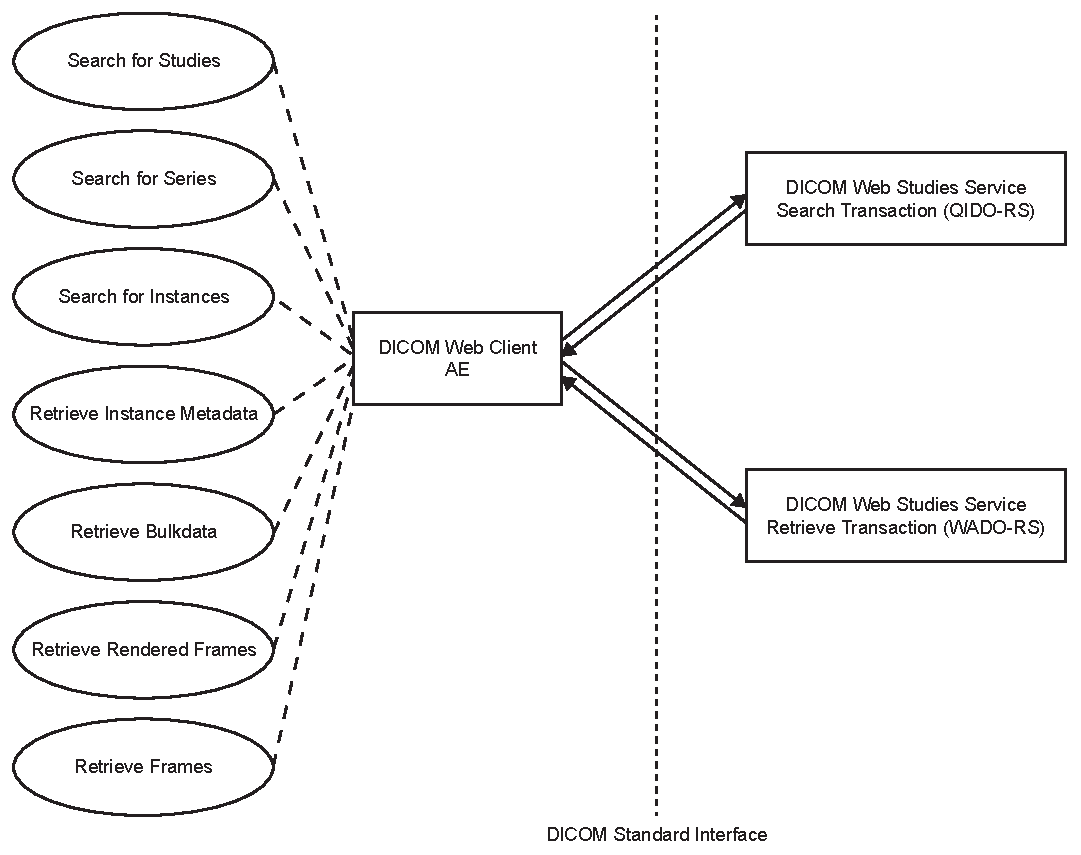
\includegraphics[width=\textwidth]{./figures/application-data-flow.pdf}
  \caption{Application Data Flow Diagram}
  \label{figure:1}
\end{figure}

\subsubsection{Functional Definition of AEs}

\paragraph{Functional Definition of ``DICOM Web Client''}

The \emph{dicomweb-client} library is a \gls{HTTP} client library that provides an \gls{API} to query, retrieve, and store \gls{REST}ful resources using the DICOM Web Studies Service.
The \emph{Slim} application uses this library internally for handling DICOM Web Studies Service requests over \gls{HTTP}.

\subsubsection{Sequencing of Real World Activities}

\begin{figure}[h!]
  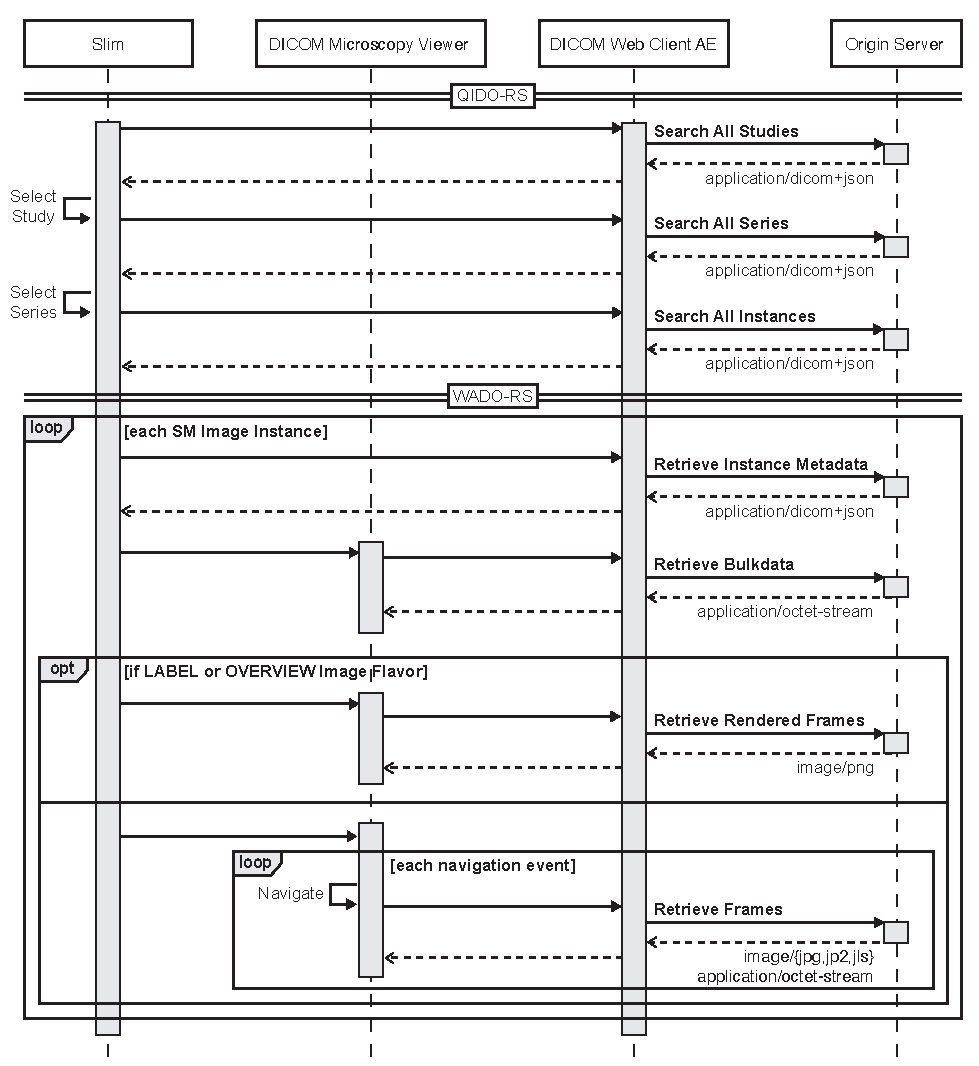
\includegraphics[width=\textwidth]{./figures/uml-sequence-diagram.pdf}
  \caption{\gls{UML} Sequence Diagram}
  \label{figure:2}
\end{figure}

\begin{itemize}
    \item{%
            The \emph{Slim} application searches for studies that contain images of modality ``SM'' using \gls{QIDO-RS} (query parameter ``ModalitiesInStudy'') and displays the list of matched study resources to the user.
    }

    \item{%
        When the user selects a study, \emph{Slim} searches for series that contain images of modality ``SM'' and that belong to selected study using \gls{QIDO-RS} (query parameters ``Modality'' and ``StudyInstanceUID'') and displays the list of matched series resources to the user.
        In addition, \emph{Slim} retrieves the metadata and rendered frames of the \texttt{OVERVIEW} image of the series (if available) using \gls{WADO-RS} and displays it to the user along with relevant metadata.
    }

    \item{%
        When the user selects a series, \emph{Slim} retrieves instance metadata for VL Whole Slide Microscopy Image instances that belong to the selected series using \gls{WADO-RS} and interprets the metadata to determine the image pyramid structure.
        \emph{Slim} further retrieves the ICC Profile for each \texttt{VOLUME} image to allow for subsequent color correction of image frames.
        In addition, \emph{Slim} retrieves the rendered frames of the \texttt{LABEL} image and the frames of the lowest resolution \texttt{VOLUME} (or \texttt{THUMBNAIL}) image of the selected series using \gls{WADO-RS} and displays the images to the user.
        \emph{Slim} also displays relevant metadata about the specimen that is the imaging target and the equipment that acquired the images.
    }

    \item{%
        When the user navigates through the multi-resolution image pyramid (e.g., via pan or zoom events), \emph{Slim} automatically retrieves frames of the \texttt{VOLUME} image of the selected series using \gls{WADO-RS} for the current slide coordinate position, decodes the frames using the appropriate codec, transforms the decoded frames using the corresponding ICC profile, and displays the transformed frames to the user.
    }
\end{itemize}

\subsection{AE Specifications}

\subsubsection{``DICOM Web Client''}

The \emph{DICOM Web Client} is a user agent for DICOM Web Services.
It supports the Search, Retrieve, and Store transactions of the Studies Service.

\paragraph{Restful Services Specifications}

\subparagraph{Retrieve Transaction of the Studies Service (WADO-RS)}

\begin{itemize}
    \item Study
    \item Study Metadata
    \item Study Bulkdata
    \item Series
    \item Series Metadata
    \item Series Bulkdata
    \item Rendered Series
    \item Instance
    \item Instance Metadata
    \item Instance Bulkdata
    \item Rendered Instance
    \item Frames
    \item Rendered Frames
    \item Bulkdata
\end{itemize}

\subparagraph{Search Transaction of the Studies Service (QIDO-RS)}

\begin{itemize}
    \item All Studies
    \item Study
    \item Study's Series
    \item Study's Instances
    \item All Series
    \item Series
    \item Series' Instances
    \item All Instances
    \item Instance
\end{itemize}

\subparagraph{Store transaction of the Studies Service (QIDO-RS)}

\begin{itemize}
    \item All Studies
    \item Study
\end{itemize}

\end{document}
